\documentclass[10pt,twocolumn,letterpaper]{article}
\usepackage[T1]{fontenc}
\usepackage[utf8]{inputenc}
\usepackage{mathpazo}
\usepackage{textcomp}
\usepackage[letterpaper,left=91.8pt,textwidth=428.4pt,top=86pt,textheight=630pt,headheight=12pt,headsep=27pt,columnsep=20pt]{geometry}
\usepackage{fancyhdr}
\usepackage{titlesec}
\usepackage{graphicx}
\usepackage{booktabs}
\usepackage{tabularx}
\usepackage{array}
\usepackage[labelfont=bf,textfont=it,labelsep=colon,font=small,format=hang]{caption}
\usepackage{enumitem}
\usepackage{microtype}
\usepackage{xcolor}

% Running head (footer is stamped later by the issue pipeline)
\pagestyle{fancy}
\fancyhf{}
\fancyhead[L]{\small\itshape Maternal healthcare network spatial impedance}
\fancyhead[R]{\small JMN Journal of Medical Sciences}
\renewcommand{\headrulewidth}{0.4pt}
\fancypagestyle{plain}{\fancyhf{}\fancyhead[L]{\small\itshape Maternal healthcare network spatial impedance}\fancyhead[R]{\small JMN Journal of Medical Sciences}}

% Section style: "I. Introduction" in small caps
\renewcommand{\thesection}{\Roman{section}}
\titleformat{\section}{\large\scshape}{\thesection.}{0.5em}{}
\titlespacing*{\section}{0pt}{14pt}{8pt}
\titleformat{\subsection}{\normalsize\bfseries}{}{0pt}{}
\titlespacing*{\subsection}{0pt}{9pt}{4pt}
\newcommand{\backhead}[1]{\par\vspace{7pt}\noindent{\bfseries #1}\par\vspace{2pt}\noindent\ignorespaces}

\renewcommand{\cite}[1]{\textsuperscript{#1}}
\setlength{\parindent}{1.5em}
\setlength{\parskip}{0pt}
\renewcommand{\arraystretch}{1.25}
\setlist[enumerate]{leftmargin=2.2em,label={[\arabic*]},itemsep=6pt,topsep=4pt}

\begin{document}
\twocolumn[{%
\begin{center}
{\large\scshape Original Article}\\[10pt]
{\fontsize{14.9}{17}\selectfont\bfseries Geospatial Network Analysis of Maternal Healthcare Access\\ and Travel Impedance in South 24 Parganas District, West Bengal\par}
\vspace{12pt}
Shuvajit Roy\textsuperscript{1$\ast$}, Rajesh Nandi\textsuperscript{2}, Anurag Mondal\textsuperscript{3}\\[8pt]
\begin{minipage}{0.86\textwidth}\footnotesize
\textsuperscript{1}Assistant Professor, Department of Community Medicine, JMN Medical College, Chakdaha (ORCID: 0009-0008-2359-3626)\\
\textsuperscript{2}Senior Resident, Department of Community Medicine, VVMC \& Safdarjung Hospital, New Delhi (ORCID: 0009-0008-3611-9990)\\
\textsuperscript{3}Senior Resident, Department of Community and Family Medicine, All India Institute of Medical Sciences, Guwahati (ORCID: 0009-0000-4508-7291; Email: dranuragmondal@yahoo.com)
\end{minipage}
\end{center}
\vspace{6pt}
\noindent\rule{\textwidth}{0.4pt}\par\vspace{6pt}
\noindent{\bfseries Abstract}\par\vspace{2pt}
\noindent{\bfseries Background:} Geographic disparities in access to emergency obstetric care contribute heavily to maternal mortality. Spatial barriers often delay life-saving clinical interventions.
{\bfseries Aims \& Objectives:} This study aimed to model the travel network impedance from localized population centers to tertiary and secondary referral health facilities in South 24 Parganas, West Bengal.
{\bfseries Methodology:} A secondary spatial data analysis was conducted for the South 24 Parganas district. The geographical coordinates bounded the region between 21\textdegree\,29$'$\,N to 22\textdegree\,33$'$\,N latitude and 88\textdegree\,3$'$\,E to 89\textdegree\,5$'$\,E longitude. Eight population nodes and five institutional health hubs were mapped. QGIS software v~3.36 was used to calculate travel time matrices using existing road and waterway network vector layers. Bed counts and local population densities served as core attribute variables.
{\bfseries Results:} The calculated travel costs from population nodes to the closest facilities varied significantly across the geographic landscape. The minimum travel impedance recorded was 19.55 minutes. The maximum recorded travel impedance reached 125.15 minutes. Remote deltaic sectors demonstrated extreme transit times to higher-order health facilities.
{\bfseries Conclusion:} Severe spatial constraints restrict healthcare access for maternal populations within remote hubs of South 24 Parganas. Targeted infrastructure investments and strategic placement of emergency obstetric care facilities are crucial to bridge these geographic gaps.\par\vspace{6pt}
\noindent{\bfseries Key Words:} Geographic Information Systems, Health Services Accessibility, Maternal Health Services, Maternal Mortality, Travel Time\par\vspace{6pt}
\noindent{\bfseries Key Message:} Geospatial network modeling reveals critical gaps and extreme travel-time variation --- up to 125 minutes --- for maternal populations accessing secondary and tertiary referral health hubs in South 24 Parganas.\par
\vspace{6pt}\noindent\rule{\textwidth}{0.4pt}\par\vspace{4pt}
\begin{center}\begin{minipage}{0.883\textwidth}\small\raggedright
{\bfseries Corresponding Author:} Dr. Shuvajit Roy, Department of Community Medicine, JMN Medical College, Chakdaha\\
{\bfseries Ethics Committee Clearance:} Not applicable --- secondary spatial data analysis with no individual human participant identifiers or clinical records accessed (as stated in the manuscript)\\
{\bfseries Source(s) of Support:} Nil (as stated in the manuscript)\\
{\bfseries Conflict of Interest:} None declared (as stated in the manuscript)\\
{\bfseries How to cite this article:} Roy S, Nandi R, Mondal A. Geospatial network analysis of maternal healthcare access and travel impedance in South 24 Parganas district, West Bengal. JMN J Med Sci. 2026 Jan--Jun;2(1):10--16.
\end{minipage}\end{center}
}]
\clearpage

\section{Introduction}
Maternal mortality remains a significant global public health concern.\cite{1} Type II delay in reaching an appropriate medical facility is a major driver of preventable maternal deaths.\cite{2,3} Spatial distance and poor transport infrastructure aggravate these barriers.\cite{4} This problem is particularly acute in developing countries and rural sub-regions.\cite{5}

The district of South 24 Parganas, with an approximate maternal mortality ratio of 110 per one lakh live births, has unique and complex geographical terrains.\cite{6} The deltaic region contains massive networks of rivers, creeks, and waterways.\cite{7} This estuarine terrain hinders the continuous development of standard road infrastructure. Consequently, pregnant women residing in these remote pockets face immense physical challenges during medical emergencies. They must navigate fragmented roads and seasonal river transport systems to reach healthcare facilities.\cite{8}

Traditional administrative planning often overlooks real-world transit layouts.\cite{9} Straight-line distance measurements do not represent true travel impedance over complex terrains.\cite{10} Geographic Information Systems (GIS) provide advanced tools to address this limitation.\cite{8} Network analysis techniques calculate precise travel times along actual transport vectors.\cite{10} These models incorporate physical barriers, road classes, and transport speeds.\cite{9} Thus, spatial modeling offers a realistic assessment of maternal healthcare accessibility.

A detailed evaluation of the existing referral network is highly necessary.\cite{8} The evidence might allow health administrators to optimize resource distribution.\cite{5} It also helps in placing emergency obstetric care facilities strategically.\cite{3} Therefore, this study was conceptualized to fill the existing gaps in regional transport planning for maternal health. The study aimed to analyze the spatial network accessibility and determine travel time impedance from various population centers to designated secondary and tertiary healthcare hubs in the South 24 Parganas district.

\section{Materials and Methods}
\subsection{Study Design and Study Area}
This study was a secondary data analysis using geospatial modeling techniques. It was conducted for the South 24 Parganas district located in West Bengal, India. The geographic boundaries of the study area extend from 21\textdegree\,29$'$\,N to 22\textdegree\,33$'$\,N latitude and 88\textdegree\,3$'$\,E to 89\textdegree\,5$'$\,E longitude.\cite{6} This district includes a mix of peri-urban plains and the unique riverine tracts of the Sundarbans delta.\cite{7} (Figure~1)

\begin{figure*}[!t]
\centering
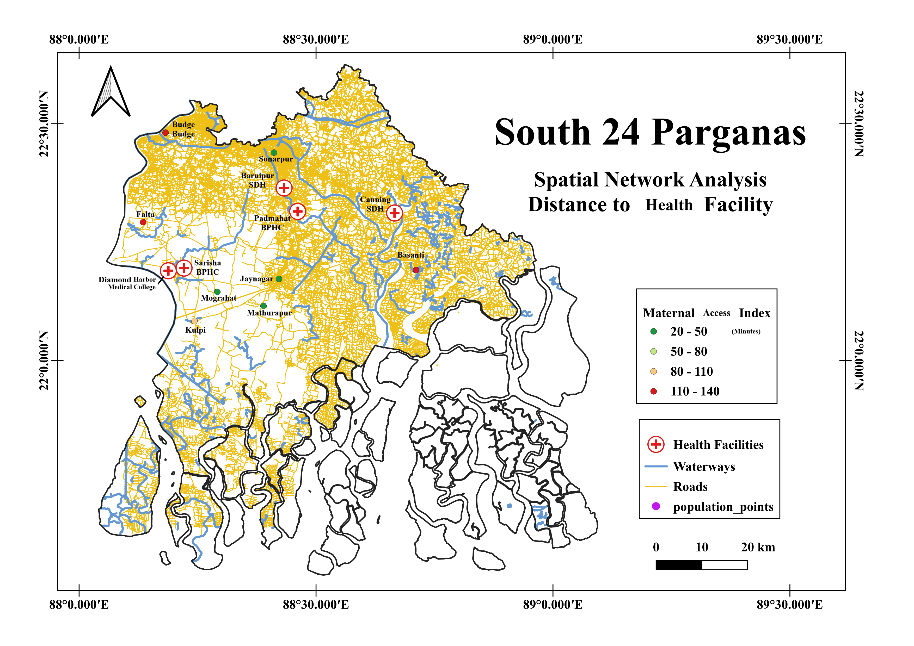
\includegraphics[width=0.74\textwidth]{fig1.png}
\caption{Spatial Network Analysis and Travel Distance to Health Facilities in South 24 Parganas.}
\end{figure*}

\subsection{Network Nodes and Hubs}
The spatial network model incorporated specific geographic points to assess travel friction.\cite{9} Eight distinct population clusters were selected and designated as origin nodes. These nodes represented major community settlements across the district geography. The selected nodes included Budge Budge, Sonarpur, Jaynagar, Mograhat, Mathurapur, Kulpi, Falta, and Basanti. Five primary institutional health facilities were selected and designated as destination hubs. These hubs included Diamond Harbor Medical College, Baruipur Sub-Divisional Hospital (SDH), Canning Sub-Divisional Hospital (SDH), Sarisha Block Primary Health Centre (BPHC), and Padmahat Block Primary Health Centre (BPHC). (Figure~1)

\subsection{Study Variables and Data Sources}
Multiple spatial and non-spatial variables were integrated into the analysis database. The primary non-spatial attribute was total bed counts at each health facility hub.\cite{6} Local population numbers within each settled locality node were included as a demand variable. The primary spatial data layers consisted of road networks, navigable waterways, and point locations of health hubs. The secondary spatial layers, transport networks, and demographic variables were sourced from official public domain repositories and institutional health records.

\subsection{Data Analysis and Spatial Modeling}
Spatial network analysis was executed utilizing open-source QGIS software version 3.36. It was used to compile the geographic database and run network simulations. A digital network graph was constructed using the vector road networks and waterway layers. Travel speeds were assigned to different road categories based on standard transport guidelines. Waterway transit parameters were added to represent ferry crossings in deltaic zones.

The Network Analysis toolbox was utilized to run an origin-destination cost matrix.\cite{9} The algorithm calculated the shortest travel paths along the network vectors.\cite{10} The accumulated travel time in minutes was computed from each of the eight origin nodes to each of the five destination hubs. The mathematical costs accounted for land-water transitions and topological connectivity. The resulting matrix values were mapped to produce a Maternal Access Index layout. The findings were visually represented using a graded colour scheme to indicate variations in transit times across the district.

The accumulated travel time in minutes was computed from each of the eight origin nodes to each of the five destination hubs to establish a comprehensive multi-destination impedance matrix. Subsequently, a secondary proximity filter was applied to isolate and map only the single least time-consuming path from each origin node to its nearest accessible healthcare facility.

\subsection{Ethical Considerations}
This research was based entirely on the analysis of secondary data layers. The dataset did not contain any individual human participant identifiers. No clinical records or personal health information were accessed during the data compilation. Therefore, this study did not require any formal ethical clearance or institutional review board permission.

\section{Results}
The spatial distribution of health facilities and the travel time categories across South 24 Parganas were mapped systematically. The geographic layout of transport vectors, waterways, and facility catchments is shown in Figure~1.

The network analysis quantified the travel impedance values between all nodes and hubs. The complete matrix of travel times in minutes is presented in Table~1.

\begin{table*}[!t]
\centering
\caption{Travel Time Impedance Matrix from Population Nodes to Health Hubs (Minutes)}
\vspace{2pt}
\small
\begin{tabularx}{\textwidth}{@{}c l *{5}{>{\centering\arraybackslash}X}@{}}
\toprule
\textbf{Origin ID} & \textbf{Population Node} & \textbf{Hub 1: Diamond Harbor Medical College} & \textbf{Hub 2: Baruipur SDH} & \textbf{Hub 3: Canning SDH} & \textbf{Hub 4: Sarisha BPHC} & \textbf{Hub 5: Padmahat BPHC} \\
\midrule
1 & Budge Budge & 33.83 & 76.17 & 125.15 & 40.75 & 79.87 \\
2 & Sonarpur & 25.82 & 79.17 & 99.30 & 19.55 & 70.77 \\
3 & Jaynagar & 30.67 & 93.64 & 109.15 & 28.46 & 80.65 \\
4 & Mograhat & 75.87 & 70.16 & 119.46 & 82.79 & 83.29 \\
5 & Mathurapur & 89.82 & 19.95 & 64.32 & 89.58 & 33.07 \\
6 & Kulpi & 54.04 & 50.57 & 67.65 & 47.20 & 37.58 \\
7 & Falta & 53.72 & 64.75 & 80.27 & 46.88 & 51.76 \\
8 & Basanti & 120.84 & 77.61 & 35.19 & 114.00 & 69.74 \\
\bottomrule
\end{tabularx}
\end{table*}

The Maternal Access Index is divided into four main travel time tiers. The green points show the shortest travel times between 20 and 50 minutes. The light green points indicate moderate travel times between 50 and 80 minutes. The orange points highlight high travel times between 80 and 110 minutes. The red points mark extreme travel times ranging from 110 to 140 minutes. (Figure~1)

The lowest travel time recorded in the entire network is 19.55 minutes. This minimum time occurs from the origin node 2 to the destination hub 4. The highest travel time recorded in the network is 125.15 minutes. This maximum impedance occurs from origin node 1 to destination hub 3. Origin node 8 shows a low travel time of 35.19 minutes to destination hub 3. However, origin node 8 shows an extreme travel time of 120.84 minutes to destination hub 1. Origin node 4 maintains a travel time above 70 minutes across all five available destination hubs. (Table~1)

The time-optimized spatial network pathway analysis mapped the actual physical transit pathways along the road and waterway infrastructure of the South 24 Parganas district. The multi-destination geographic distribution model highlights a stark regional imbalance. (Figure~2) Figure~2a describes the exhaustive network of all potential spatial paths. The time-optimized pathways in Figure~2b demonstrate that rapid healthcare access remains localized. The most efficient transit routes (under 29 minutes) are heavily restricted to the western and northwestern perimeters, leaving communities adjacent to the southern deltaic networks isolated, facing significantly higher travel times to reach secondary or tertiary clinical infrastructure.

\begin{figure*}[!t]
\centering
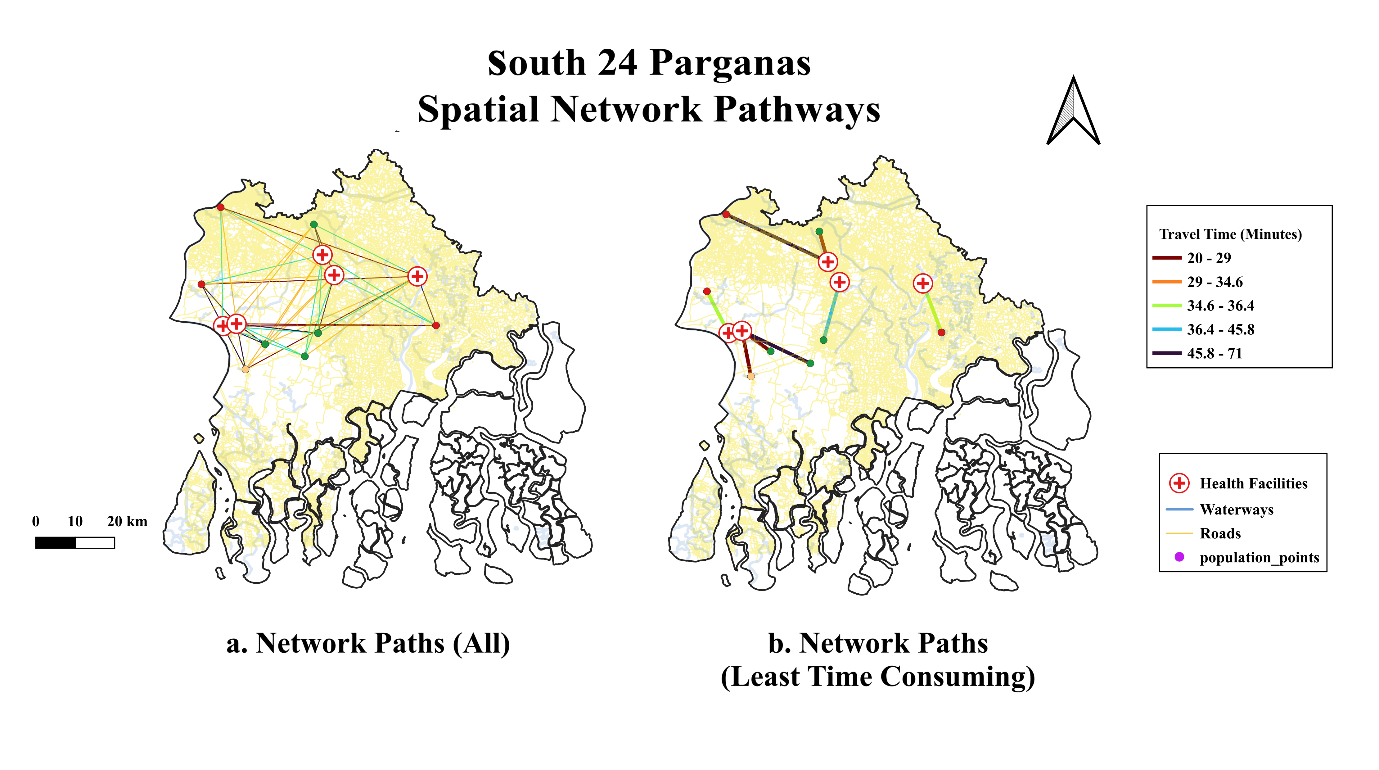
\includegraphics[width=\textwidth]{fig2.png}
\caption{Time-Optimized Spatial Network Path Analysis and Geographic Accessibility Tiers across South 24 Parganas, West Bengal.}
\end{figure*}

\section{Discussion}
The main objective of this study was to analyze spatial network accessibility and determine travel time impedance from population nodes to designated health hubs in South 24 Parganas. The findings showed a wide variation in travel impedance across the district.

Several factors explain the significant differences in travel times. The estuarine geography of South 24 Parganas creates natural obstacles for land transport.\cite{7} Localities like Basanti are separated from major urban centers by rivers and creeks. Relying on ferry connections increases transit times significantly.\cite{6} This reliance explains the high travel cost of 120.84 minutes from Basanti to Diamond Harbor Medical College. Conversely, sectors with contiguous highway networks show much lower travel impedance. For example, Sonarpur shows a short travel time of 19.55 minutes to Sarisha BPHC due to better road connectivity. Fragmented infrastructure directly compromises maternal health outcomes.\cite{5} Long transit times prolong the second delay during obstetric emergencies.\cite{2} This delay increases the risk of birth complications and maternal mortality.\cite{4} Pockets facing travel times above 80 minutes require urgent attention. These high-impedance zones leave pregnant women vulnerable when complications arise.\cite{8}

Subsequently, when the network is optimized to model transit strictly to the closest available health facility (Figure~2b), a different layer of spatial inequality emerges. Even under this ideal-case scenario, the safety net is not uniform; while western border populations enjoy highly efficient access within 29 minutes, other northern and sub-deltaic communities still experience localized infrastructure friction and bottlenecks that stretch nearest-facility transit up to 71 minutes. This implies that proximity on a map does not automatically equate to rapid clinical access when the underlying road vectors are fragmented.

This study used actual road and waterway network paths instead of simple straight-line distances. This approach provided a realistic model of travel impedance over difficult deltaic terrain. The dual-model approach of integrating a comprehensive multi-destination matrix alongside a proximity-filtered nearest-hub analysis significantly enhances the accuracy and utility of the geographic model for real-world referral planning.

Thus, localities with travel times exceeding 100 minutes need immediate decentralized care options. Specialized obstetric stabilization units should be set up at riverine transit points. Multi-modal transport networks must be improved. Upgrading ferry services and building bridges will reduce travel friction significantly. Lastly, future research should incorporate seasonal variables into network models. Analyzing transit variations during heavy monsoons will provide deeper insights. Researchers should also look at how facility capacities affect patient choices. Combining spatial travel costs with clinical quality data will help optimize maternal health planning.

\section{Conclusion}
This study highlights major geographic disparities in maternal healthcare access across South 24 Parganas. Network modeling revealed that travel times to referral hubs range from under 20 minutes to over two hours. The riverine landscape creates significant transit barriers for remote communities. These findings emphasize that straight-line distance models underestimate actual travel barriers. Reducing these spatial inequities requires targeted infrastructure investments and decentralized emergency obstetric facilities. Implementing these spatial adjustments is essential to eliminating transit delays and lowering maternal mortality.

\backhead{Limitations of the Study}
The network analysis assumed static travel speeds along transport vectors. It did not account for real-time traffic congestion or seasonal weather disruptions. Monsoonal flooding often slows transit speeds or disrupts ferry services completely in the Sundarbans. Furthermore, the model did not include the use of private transport modes or emergency ambulance availability.

\backhead{Authors' Contribution}
All authors contributed substantially to this study, from conceptualization, study design, literature search, data curation and data analysis to manuscript writing and review. All of them are guarantors of this work.

\backhead{Financial Support and Sponsorship}
The authors did not receive any support from any source.

\backhead{Conflict of Interest}
The authors have no conflicts of interest regarding this work.

\backhead{Acknowledgement}
The authors are thankful to Dr. Soumalya Ray, Associate Professor, Dept. of Community Medicine, SGGGM \& CH, Uluberia, Howrah, West Bengal, India, for guiding them on the application and usage of GIS.

\backhead{Declaration of Generative AI and AI-Assisted Technologies in the Writing Process}
The authors did not use AI at any stage of this study.

\section*{\large\scshape References}
\small
\begin{enumerate}
\item Alkema L, Chou D, Hogan D, Zhang S, Moller AB, Gemmill A, et al. Global, regional, and national levels and trends in maternal mortality between 1990 and 2015, with scenario-based projections to 2030: a systematic analysis by the Maternal Mortality Estimation Inter-Agency Group. Lancet. 2016;387(10017):462-74.
\item Mullan Z. The second delay in maternal mortality. Lancet Glob Health. 2014;2(12):e673.
\item Thaddeus S, Maine D. Too far to walk: maternal mortality in context. Soc Sci Med. 1994;38(8):1091-110.
\item Gabrysch S, Campbell OM. Still too far to walk: literature review of the determinants of delivery service use. BMC Pregnancy Childbirth. 2009;9:34.
\item World Health Organization. Standards for improving quality of maternal and newborn care in health facilities. Geneva: World Health Organization; 2016.
\item Government of West Bengal. District Human Development Report: South 24 Parganas. Development and Planning Department; 2010.
\item Mondal NA, Das S. Infrastructure and development challenges in the Sundarbans region of West Bengal. Indian J Landscape Syst Ecol Stud. 2018;41(2):112-25.
\item Ray N, Jarvis CI, Camargo MT, et al. Estimating spatial accessibility to emergency obstetric care in West Bengal using geographic information systems. Int J Health Geogr. 2021;20(1):15.
\item Fiedler JL. The Kunin and Gegghegan approach to evaluate health care accessibility: a network analysis alternative. Soc Sci Med. 2012;74(4):512-20.
\item Kelly C, Hulme C, Farragher T, Clarke G. Are spatial networks accurate enough to calculate travel times to healthcare? A validation study. Int J Health Geogr. 2019;18(1):26.
\end{enumerate}
\end{document}
